\documentclass[10pt]{beamer}

% paquets pour le français
\usepackage[T1]{fontenc}
\usepackage[utf8]{inputenc}

% paquets autres
\usepackage{ulem}
\usepackage{listings}
\usepackage{xcolor}
\usepackage{hyperref}
\usepackage{graphicx}
\usepackage[figurename=Source]{caption}

% couleurs
\definecolor{light-grey}{RGB}{240,240,240}
\definecolor{dark-green}{RGB}{50, 80, 50}
\definecolor{cherry-red}{RGB}{200, 40, 40}

% theme général du diaporama
\usetheme{Madrid}
\usecolortheme[RGB={13, 87, 63}]{structure}

% configuration des zones de code
\lstset{
	backgroundcolor = \color{light-grey},  % Choose the background color
    commentstyle    = \color{dark-green},  % Highlighting comment
    keywordstyle    = \color{cherry-red},  % Highlighting keywords
    stringstyle     = \color{orange},      % Highlighting string
    inputencoding   = utf8,                % Input encoding
    extendedchars   = true,                % Extended ASCII
    breaklines      = true,                % Sets automatic line breaking
    language        = C,                   % Set language
    basicstyle      = \ttfamily\scriptsize,     % Set font size
    numbers         = left,                % Numeration
    numbersep       = 5pt,                 % Set numeration shift
    literate        =                      % Support additional characters
      {á}{{\'a}}1  {é}{{\'e}}1  {í}{{\'i}}1 {ó}{{\'o}}1  {ú}{{\'u}}1
      {Á}{{\'A}}1  {É}{{\'E}}1  {Í}{{\'I}}1 {Ó}{{\'O}}1  {Ú}{{\'U}}1
      {à}{{\`a}}1  {è}{{\`e}}1  {ì}{{\`i}}1 {ò}{{\`o}}1  {ù}{{\`u}}1
      {À}{{\`A}}1  {È}{{\'E}}1  {Ì}{{\`I}}1 {Ò}{{\`O}}1  {Ù}{{\`U}}1
      {ä}{{\"a}}1  {ë}{{\"e}}1  {ï}{{\"i}}1 {ö}{{\"o}}1  {ü}{{\"u}}1
      {Ä}{{\"A}}1  {Ë}{{\"E}}1  {Ï}{{\"I}}1 {Ö}{{\"O}}1  {Ü}{{\"U}}1
      {â}{{\^a}}1  {ê}{{\^e}}1  {î}{{\^i}}1 {ô}{{\^o}}1  {û}{{\^u}}1
      {Â}{{\^A}}1  {Ê}{{\^E}}1  {Î}{{\^I}}1 {Ô}{{\^O}}1  {Û}{{\^U}}1
      {œ}{{\oe}}1  {Œ}{{\OE}}1  {æ}{{\ae}}1 {Æ}{{\AE}}1  {ß}{{\ss}}1
      {ç}{{\c c}}1 {Ç}{{\c C}}1 {ø}{{\o}}1  {Ø}{{\O}}1   {å}{{\r a}}1
      {Å}{{\r A}}1 {ã}{{\~a}}1  {õ}{{\~o}}1 {Ã}{{\~A}}1  {Õ}{{\~O}}1
      {ñ}{{\~n}}1  {Ñ}{{\~N}}1  {¿}{{?`}}1  {¡}{{!`}}1
      {°}{{\textdegree}}1 {º}{{\textordmasculine}}1 {ª}{{\textordfeminine}}1
  }

% gestion des sections
\AtBeginSection[]{
	\begin{frame}
	\vfill
	\centering
	\begin{beamercolorbox}[sep=8pt, center]{title}
		\usebeamerfont{title}
  		\uline{\insertsectionhead}
  		\par
  	\end{beamercolorbox}
  	\vfill
  	\end{frame}
}

% gestion des blocs
\setbeamertemplate{blocks}[default]

% gestion des frames
\setbeamertemplate{frametitle continuation}{}
\setbeamersize{text margin left = 20px,text margin right = 20px} 

% informations
\author[\textit{Thomas CREUSET}]{\textit{Thomas CREUSET (11909) et Nicolas SEGALA (17862)}}
\title{\uline{Pr\'esentation de TIPE}}
\subtitle{\textit{\'Etude et optimisation d’un outil d'ing\'enierie du b\^atiment}}
\date[\textit{num\'ero de candidat  : 11909}]{}

% document
\begin{document}

	% page de titre
	\frame{\titlepage}

	% Problèmatique
	\begin{frame}
		\frametitle{\uline{Probl\'ematique}}
		\begin{block}{}
			- Quel est le potentiel gain temporel du calcul analogique par rapport à la méthode purement
numérique?\\
			- Quels sont les enjeux pratiques de sa mise en place pour la méthode des éléments
finis?
		\end{block}
	\end{frame}

	% sommaire
	\part{Sommaire}
	\begin{frame}
		\frametitle{\uline{Sommaire}}
		\tableofcontents
	\end{frame}

	% Choix du projet
	\section{Choix du projet}
	% frame 1.1
	\subsection{La construction en ville : un enjeu pour les ing\'enieurs}
	\begin{frame}
		\frametitle{\uline{Choix du projet :}}
		\framesubtitle{\textit{La construction en ville : un enjeu pour les ing\'enieurs}}
		\begin{columns}[t]
  			\begin{column}{5cm} 
				\begin{block}{}
					\uline{Objectifs de l'ing\'enieur :}
  					\begin{itemize}
						\item Stabilit\'e
						\item Durabilit\'e
						\item Accessibilit\'e
						\item Autres
					\end{itemize}
					\uline{Point d'int\'er\^et pour notre TIPE :}
					\begin{itemize}
						\item Stabilit\'e
					\end{itemize}
				\end{block}
  			\end{column}
 			\begin{column}{5cm}
 				\begin{figure}
   					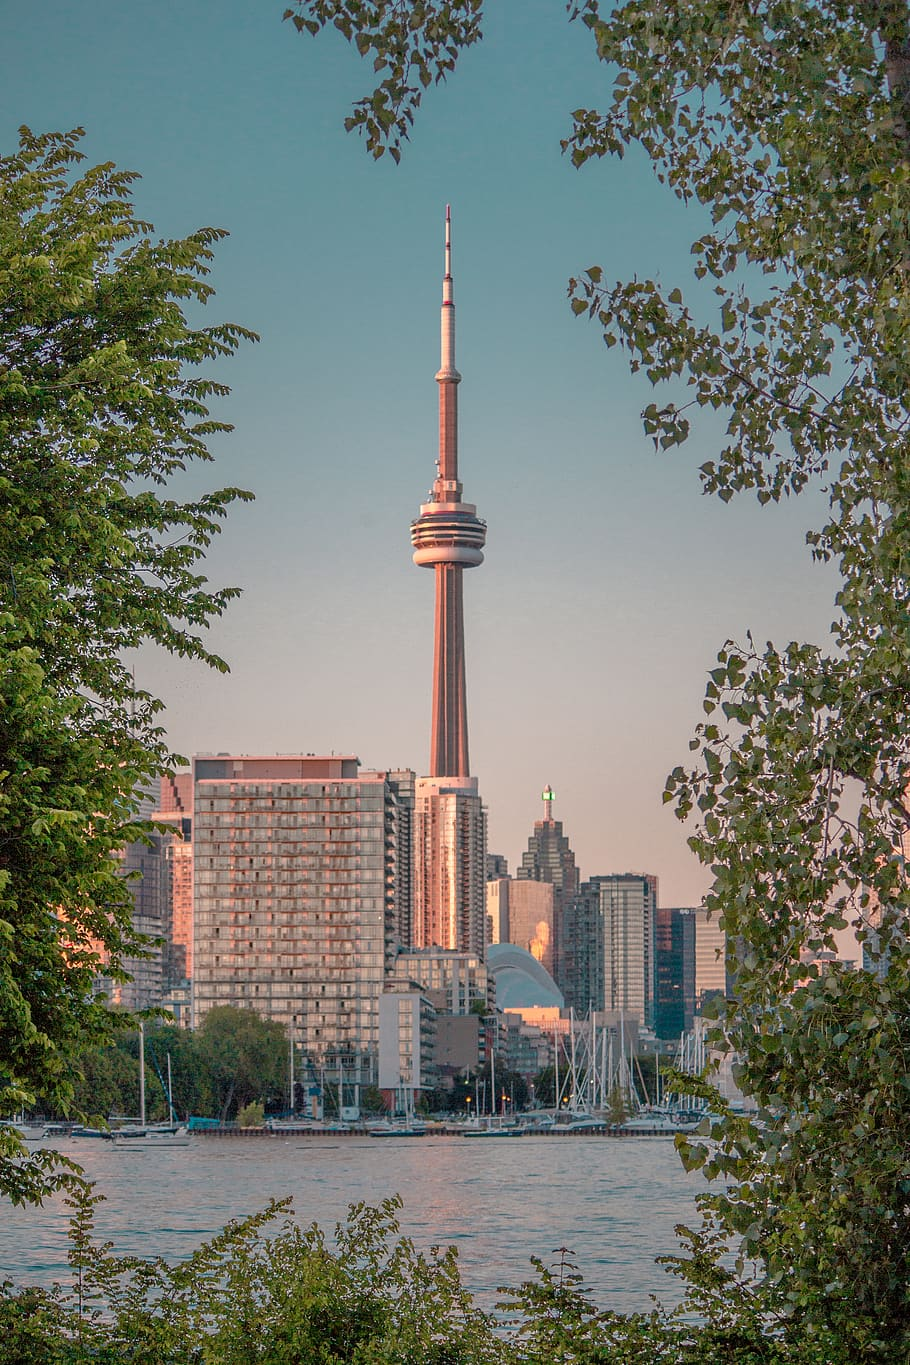
\includegraphics[scale = 0.125]{Images/city.png}
   					\caption{\href{https://www.wallpaperflare.com/city-portrait-buildings-skyscraper-tower-tall-toronto-wallpaper-eafsn}{wallpaperflare}}
				\end{figure}
			 \end{column}
 		\end{columns}
	\end{frame}
	%frame 1.2
	\subsection{Mod\'elisation informatique}
	\begin{frame}
		\frametitle{\uline{Choix du projet :}}
		\framesubtitle{\textit{Mod\'elisation informatique}}
		
		\begin{columns}[t]
  			\begin{column}{5cm} 
 				\begin{figure}
   					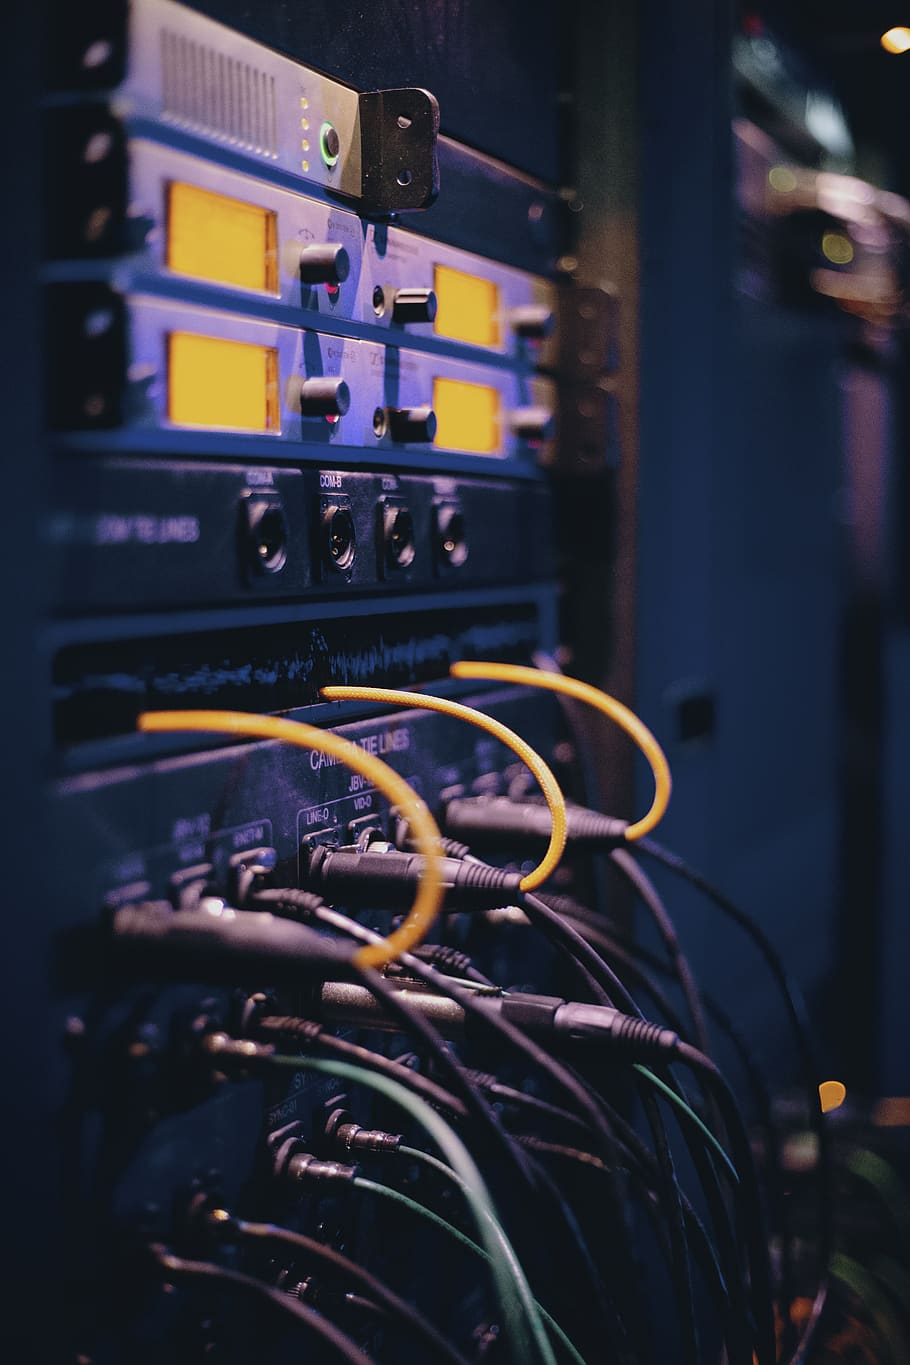
\includegraphics[scale = 0.125]{Images/cables.jpg}
   					\caption{\href{https://www.wallpaperflare.com/black-cables-connection-data-electronics-equipment-ethernet-wallpaper-aryet}{wallpaperflare}}
				\end{figure}
  			\end{column}
 			\begin{column}{5cm}
 				\begin{block}{}
 					\uline{Int\'er\^ets de la mod\'elisation informatique :}
					\begin{itemize}
						\item Co\^ut
						\item Dur\'ee
						\item Flexibilit\'e
					\end{itemize}
				\end{block}
			 \end{column}
 		\end{columns}
	\end{frame}
	
	% Méthode des éléments finis
	\section{\'Elaboration de la m\'ethode des \'el\'ements finis}
	%frame 2.1
	\subsection{M\'ethode des \'el\'ements finis}
	\begin{frame}
		\frametitle{\uline{\'Elaboration de la m\'ethode des \'el\'ements finis :}}
		\framesubtitle{\textit{M\'ethode des \'el\'ements finis}}
		\centering
		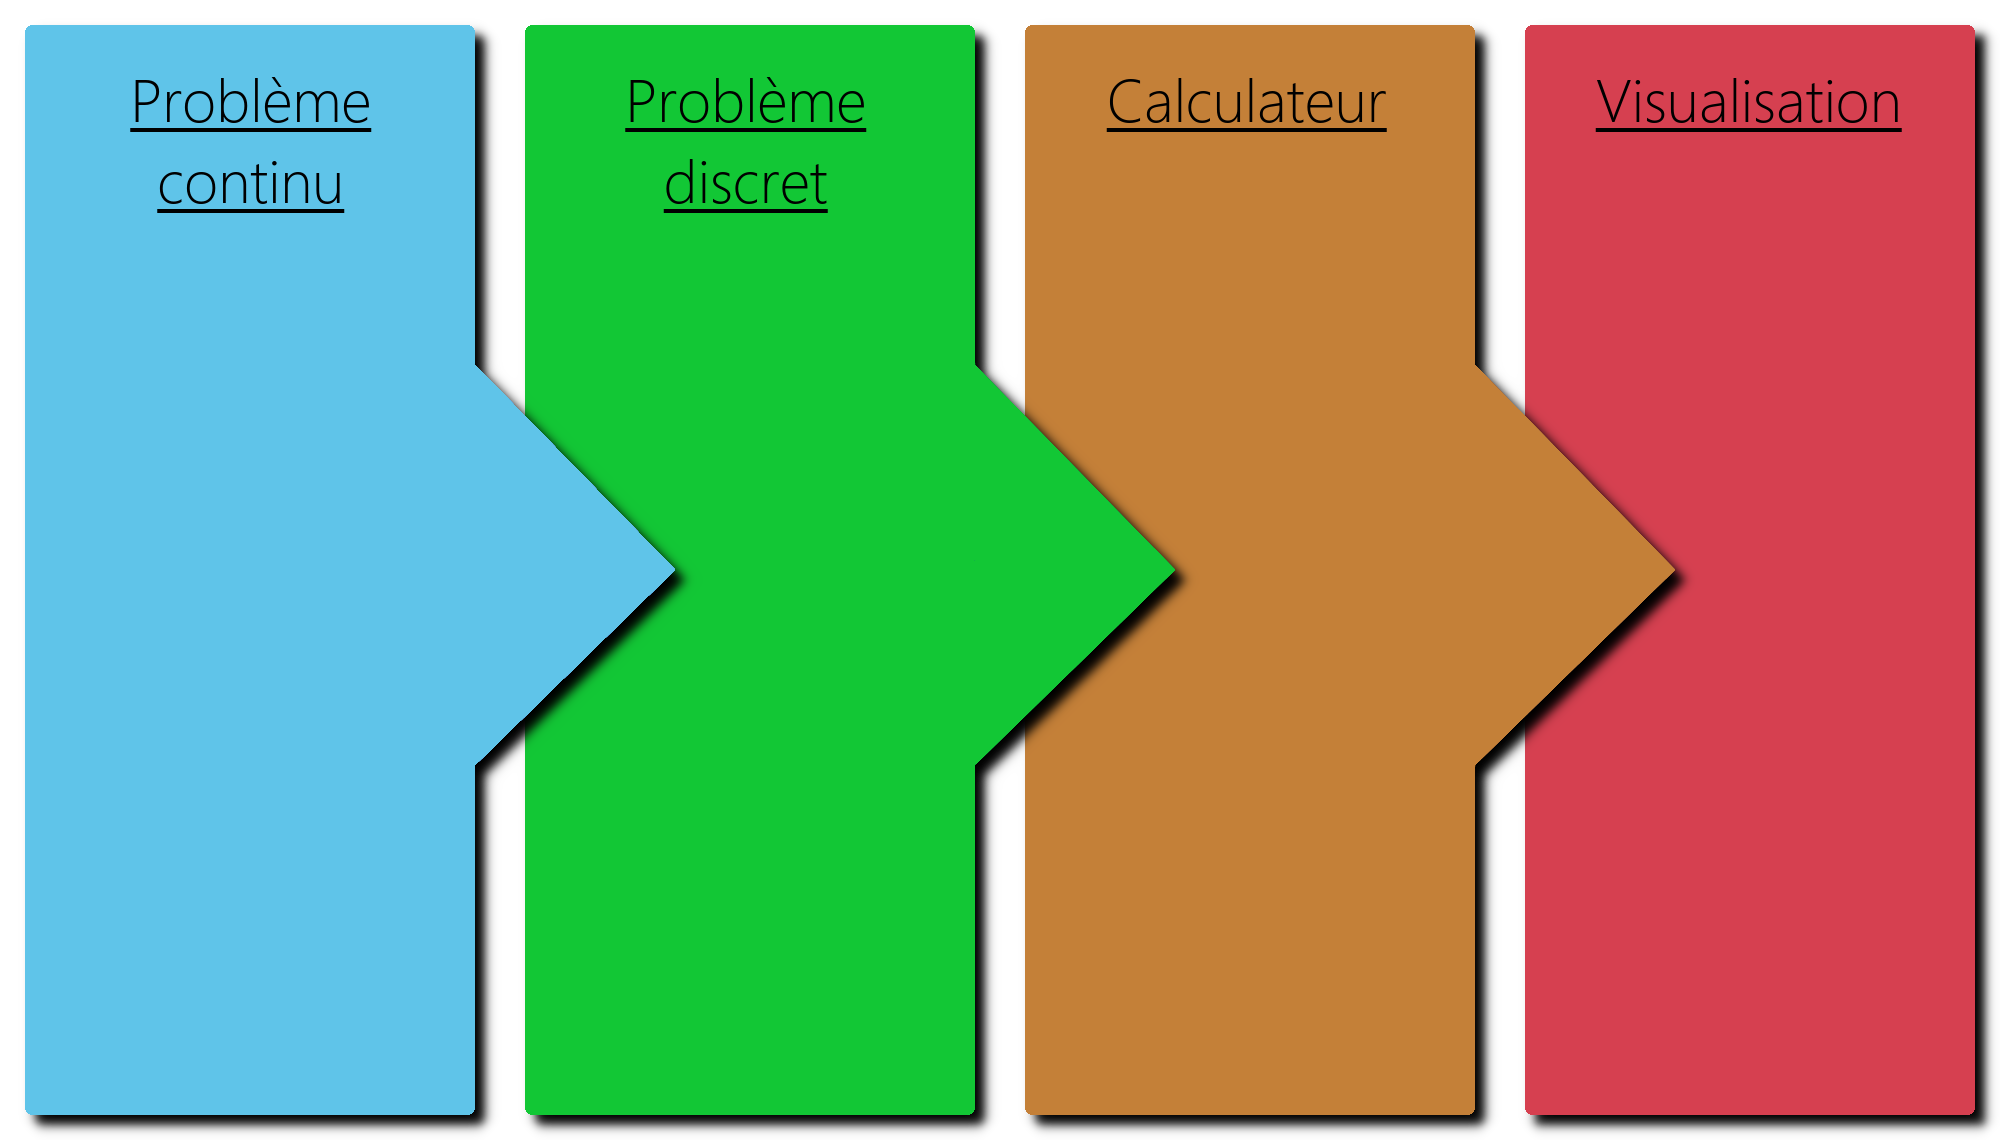
\includegraphics[scale=4.5]{Images/MethodeDesElementsFinis.png}
	\end{frame}
	% frame 2.2
	\subsection{M\'ethode des ressorts}
	\begin{frame}
		\frametitle{\uline{\'Elaboration de la m\'ethode des \'el\'ements finis :}}
		\framesubtitle{\textit{M\'ethode des ressorts}}
		\begin{columns}[t]
 			\begin{column}{5cm}
 				\begin{figure}
 				 	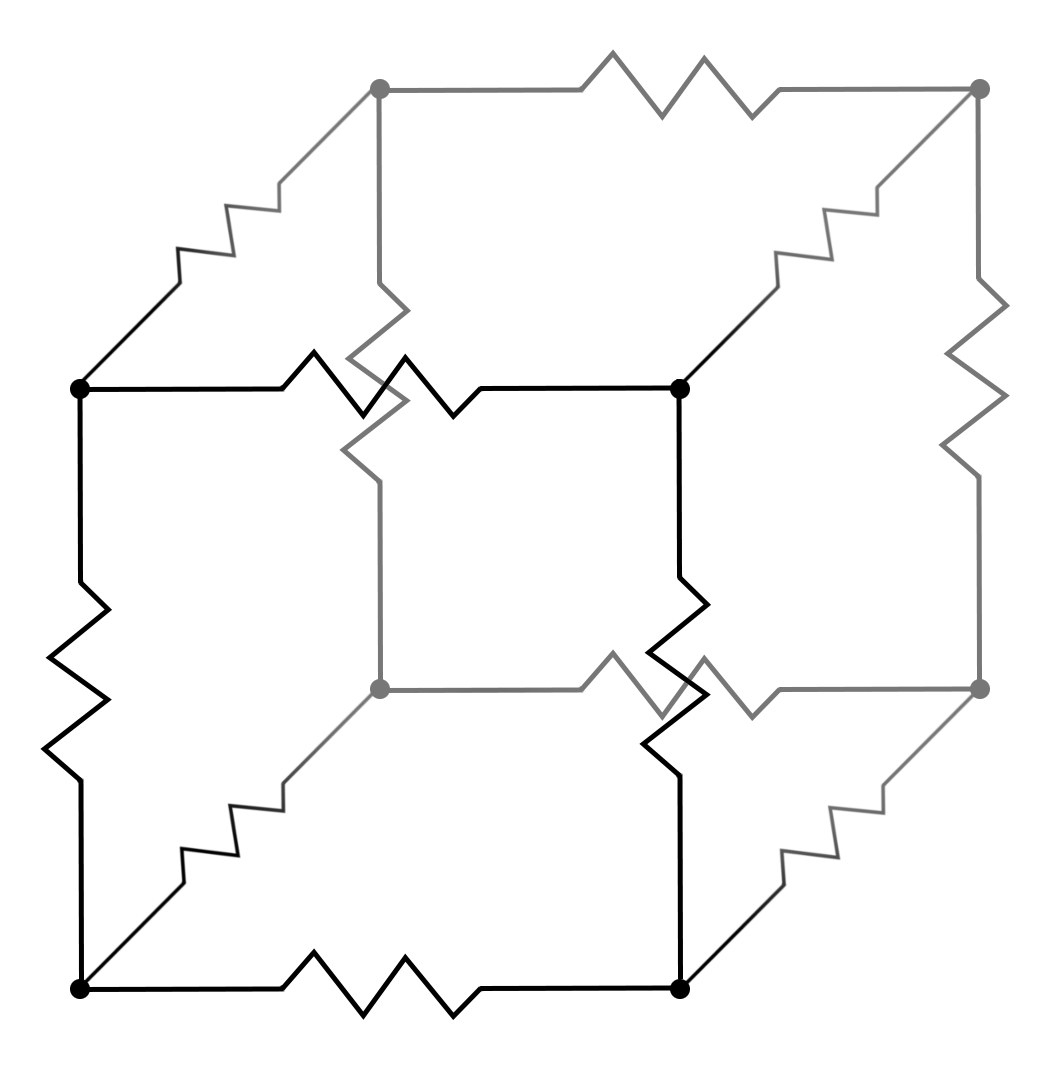
\includegraphics[scale=0.50]{Images/cubeFinal.png}
 				\end{figure}
			\end{column}
			\begin{column}{5cm}
				\begin{block}{}
					\uline{Principe :}
					\begin{itemize}
						\item Discr\'etisation en un ensemble de points reli\'es par des ressorts
						\item Mod\'elisation de l'action des ressorts par la loi de Hooke
						\item Utile pour mod\'eliser des poutres dans un b\^atiment
					\end{itemize}
				\end{block}
  			\end{column}
 		\end{columns}
	\end{frame}
	% frame 2.3
	\subsection{Loi de Hooke}
	\begin{frame}
		\frametitle{\uline{\'Elaboration de la m\'ethode des \'el\'ements finis :}}
		\framesubtitle{\textit{Loi de Hooke}}
		\begin{columns}[t]
 			\begin{column}{5cm}
 				\begin{block}{Loi de Hooke}
					\begin{equation}
  						\vec{\mathcal{F}} = - \mathit{k} \cdot \Delta \ell \cdot \vec{u}
  					\end{equation}
				\end{block}
				\begin{figure}
 				 	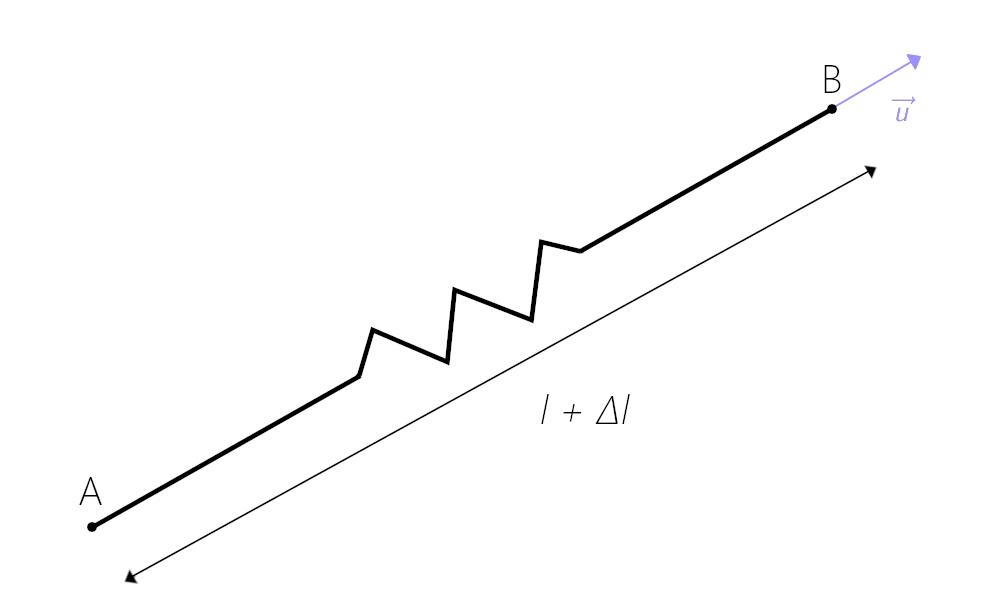
\includegraphics[scale=0.62]{Images/Hooke.png}
 				\end{figure}
			\end{column}
			\begin{column}{5cm}
				\begin{block}{Constante de raideur}
					\begin{equation}
						\mathit{k} = \frac{\mathit{A} \cdot \mathit{E}}{\mathit{L}}
					\end{equation}
					avec :\\
  					\begin{itemize}
  						\item $\mathit{A}$ : l'aire de la section de la poutre
  						\item $\mathit{E}$ : le module de Young du matériel
  						\item $\mathit{L}$ : la longueur de la poutre
  					\end{itemize}
				\end{block}
  			\end{column}
 		\end{columns}
	\end{frame}
	%frame 2.4
	\subsection{Deux \'etapes importantes}
	\begin{frame}
		\frametitle{\uline{\'Elaboration de la m\'ethode des \'el\'ements finis :}}
		\framesubtitle{\textit{Deux astuces, rotation}}
		\begin{columns}[t]
			\begin{column}{5cm}
				\begin{block}{}
					\uline{Rotation vers le cas trivial :}
  					\begin{equation}
						\begin{pmatrix}
							1 & 0 & 0 & -1 & 0 & 0 \\
							0 & 0 & 0 & 0 & 0 & 0 \\
							0 & 0 & 0 & 0 & 0 & 0 \\
							-1 & 0 & 0 & 1 & 0 & 0 \\
							0 & 0 & 0 & 0 & 0 & 0 \\
							0 & 0 & 0 & 0 & 0 & 0
						\end{pmatrix}
					\end{equation}
				\end{block}
  			\end{column}
 			\begin{column}{5cm}
 				\begin{figure}
 				 	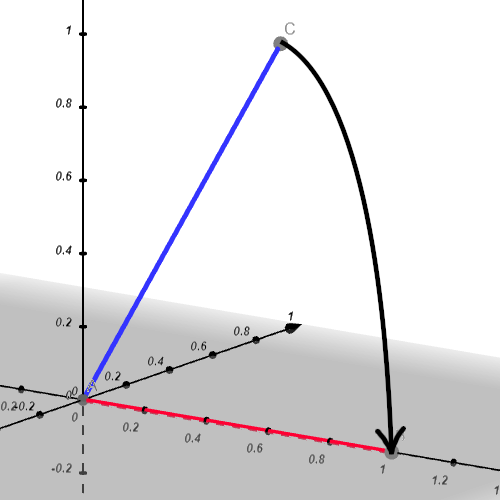
\includegraphics[scale=0.35]{Images/CasFinal.png}
 				\end{figure}
			\end{column}
 		\end{columns}
	\end{frame}
	%frame 2.5
	\begin{frame}
		\frametitle{\uline{\'Elaboration de la m\'ethode des \'el\'ements finis :}}
		\framesubtitle{\textit{Deux \'etapes importantes, calcul de la solution }}
		\begin{block}{Tri des noeuds (Conditions de Dirichlet et de Neumann)}
			\begin{equation}
				\begin{pmatrix}
				F_c \\
				F_i
				\end{pmatrix}
				=
				\begin{pmatrix}
				K_1 & K_2 \\
				K_3 & K_4
				\end{pmatrix}
				\cdot
				\begin{pmatrix}
				U_i \\
				U_c
				\end{pmatrix}
			\end{equation}
		\end{block}
		\begin{block}{R\'ecup\'eration des forces et des d\'eplacements inconnus}
			\begin{align}
				&F_c = K_1 \cdot U_i + K_2 \cdot U_c\\
				&\textit{d'o\`u : } U_i = K_1^{-1} \cdot (F_c - K_2 \cdot U_c)\\
				&\textit{et : } F_i = K_3 \cdot U_i + K_4 \cdot U_c
			\end{align}
		\end{block}
	\end{frame}
	%frame 2.6
	\subsection{Affichage}
	\begin{frame}
		\frametitle{\uline{\'Elaboration de la m\'ethode des \'el\'ements finis :}}
		\framesubtitle{\textit{Affichage}}
		\uline{Deux exemples de rendu par l'algorithme du peintre :}
		\begin{columns}[t]
			\begin{column}{5cm}
				\begin{figure}
 				 	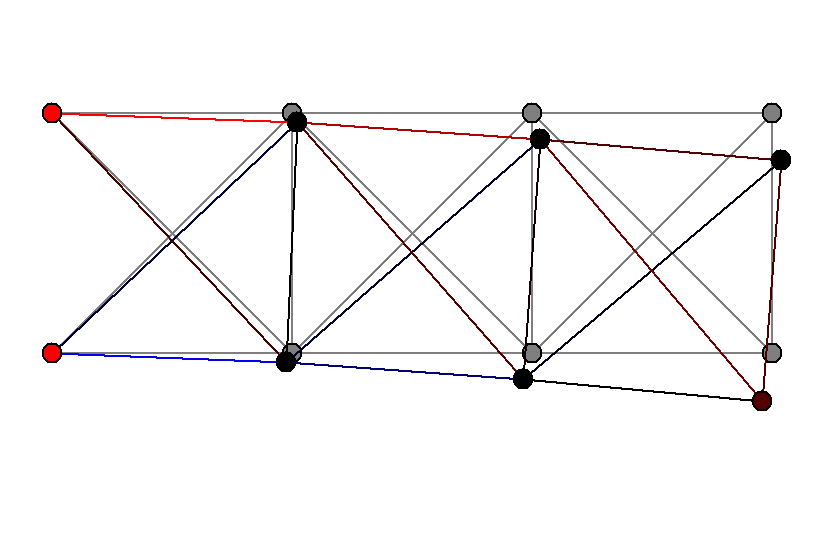
\includegraphics[scale=0.26]{Images/2D_exemple.png}
 				\end{figure}
  			\end{column}
 			\begin{column}{5cm}
 				\begin{figure}
 				 	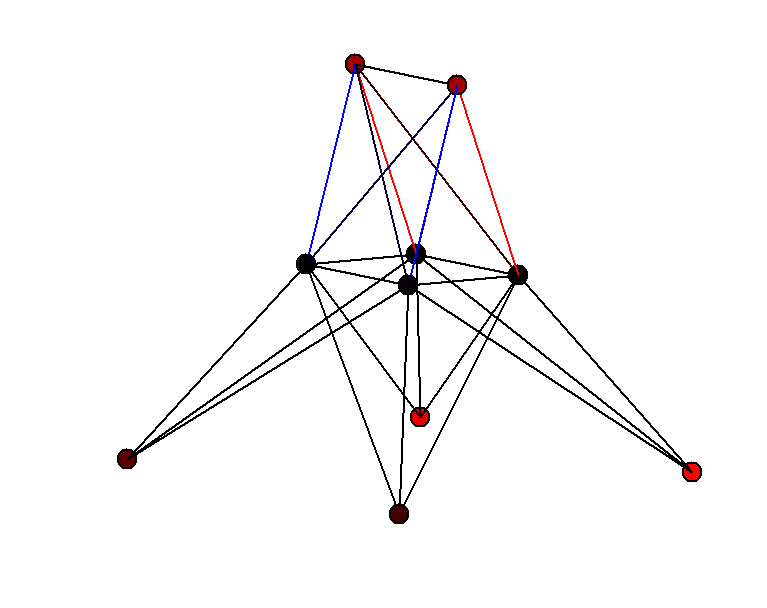
\includegraphics[scale=0.26]{Images/3D_exemple.png}
 				\end{figure}
			\end{column}
 		\end{columns}
 		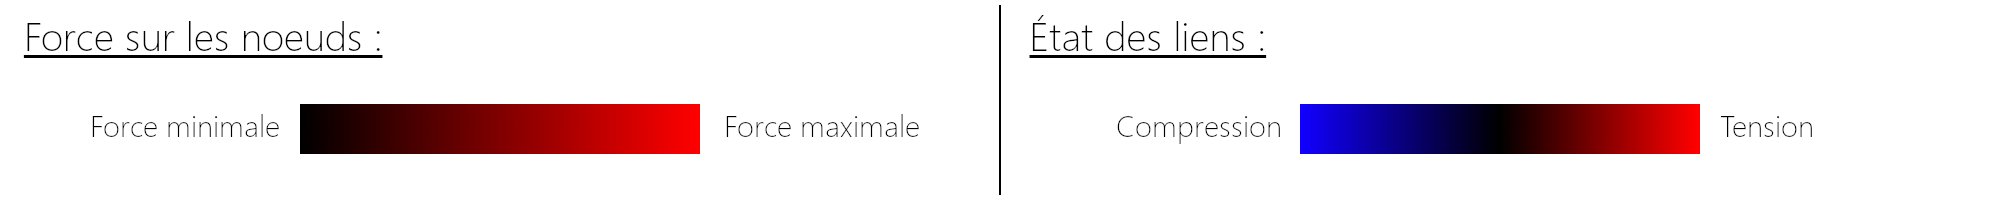
\includegraphics[scale=0.69]{Images/legende.png}
	\end{frame} 

	% Optimisation
	\section{Optimisation}
	% frame 3.1
	\subsection{Calculs analogique, int\'er\^ets}
	\begin{frame}
		\frametitle{\uline{Optimisation :}}
		\framesubtitle{\textit{Calculs analogique, int\'er\^ets}}
		\uline{Int\'er\^ets du calcul analogique :}
		\begin{itemize}
			\item parall\'elisation et quasi-linéarisation des produits matriciels : $O(n^{2.38})$ avec l'algorithme de Strassen à $O(n^2)$ en analogique
			\item ancienne m\'ethode fiable
			\item domaine qui sucite un regain d'int\'er\^et (Mythic)
		\end{itemize}
	\end{frame}
	%frame 3.2
	\subsection{Retours exp\'erimentaux}
	\begin{frame}
		\frametitle{\uline{Optimisation :}}
		\framesubtitle{\textit{Retours exp\'erimentaux}}
		Pas encore fait
	\end{frame}
	
	% Conlusion
	\section{Conclusion}
	\begin{frame}
		\frametitle{\uline{Conclusion}}
		\centering
  		\vfill
		Algorithme d'inversion HHL (H.arrow H.assidim L.loyd) :
		\begin{quote}
			<<HHL apporte une amélioration significative, de O(n) à O(log(n)).>>\footnote{\textit{L’apport des technologies quantiques en intelligence artificielle : vers une acculturation et une compr\'ehension des enjeux du quantique pour l’arm\'ee de l’air et de l’espace}, Commandant Campo Marie-\'Elisabeth, Bureau num\'erique de l’arm\'ee de l’air et de l’espace}
		\end{quote}
	\end{frame}
	
	% Annexes
	\section{Annexes}
	% partie C
	\subsection{Code C}
	\begin{frame} [allowframebreaks]
		\frametitle{\uline{Annexes :}}
		\framesubtitle{\textit{Code C : standard\_lib.h}}
		\lstinputlisting{Code/C/standard_lib.h}
	\end{frame}
	\begin{frame}[allowframebreaks]
		\frametitle{\uline{Annexes :}}
		\framesubtitle{\textit{Code C : module\_matrice.h}}
		\lstinputlisting{Code/C/module\_matrice.h}
	\end{frame}
	\begin{frame}[allowframebreaks]
		\frametitle{\uline{Annexes :}}
		\framesubtitle{\textit{Code C : module\_matrice.c}}
		\lstinputlisting{Code/C/module\_matrice.c}
	\end{frame}
	\begin{frame}[allowframebreaks]
		\frametitle{\uline{Annexes :}}
		\framesubtitle{\textit{Code C : main.c}}
		\lstinputlisting{Code/C/main.c}
	\end{frame}
	% partie C
	\subsection{Code Ocaml}
	\begin{frame} [allowframebreaks]
		\frametitle{\uline{Annexes :}}
		\framesubtitle{\textit{Code Ocaml : Affichage\_FEM\_3D.ml}}
		\lstinputlisting[language = caml]{Code/Ocaml/Affichage_FEM_3D.ml}
	\end{frame}
\end{document}

